\documentclass[11pt,twoside,titlepage,a4paper]{article}
%%%%%%%%%%%%%%%%%%%%%%%%%%%%%%%%%%%%%%%%%
%				PAQUETES				%
%%%%%%%%%%%%%%%%%%%%%%%%%%%%%%%%%%%%%%%%%
\usepackage{amsmath} % Matemáticas
\usepackage{amsfonts} % Letras caligráficas para matemáticas
\usepackage{enumitem} % Opciones de personalización de listas
\usepackage{fancyhdr} % Encabezados/pies de páginas
\usepackage[a4paper]{geometry} % Márgenes
\usepackage{mathtools} % Matemáticas extra
\usepackage{newtxsf} % Tipografía
\usepackage{listings} % Código

%%%%%%%%%%%%%%%%%%%%%%%%%%%%%%%%%%%%%%%%%
%			  TIPOGRAFÍA				%
%%%%%%%%%%%%%%%%%%%%%%%%%%%%%%%%%%%%%%%%%
\usepackage[T1]{fontenc}
\usepackage[sfdefault,scaled=.85]{FiraSans}

%%%%%%%%%%%%%%%%%%%%%%%%%%%%%%%%%%%%%%%%%
%				MÁRGENES				%
%%%%%%%%%%%%%%%%%%%%%%%%%%%%%%%%%%%%%%%%%
\geometry{
	left=2.5cm,
	right=2.5cm,
	bottom=2.5cm
}

%%%%%%%%%%%%%%%%%%%%%%%%%%%%%%%%%%%%%%%%%
%				  CÓDIGO				%
%%%%%%%%%%%%%%%%%%%%%%%%%%%%%%%%%%%%%%%%%
\lstset{
	basicstyle=\footnotesize\ttfamily,
	breaklines=true,
	language=C++,
	frame=single,
	numbers=left,
	numbersep=5pt,
	tabsize=4,
	frame=leftline
}

%%%%%%%%%%%%%%%%%%%%%%%%%%%%%%%%%%%%%%%%%
%				COMANDOS				%
%%%%%%%%%%%%%%%%%%%%%%%%%%%%%%%%%%%%%%%%%
\renewcommand{\contentsname}{Índice} % Cambiar el título del índice
\renewcommand{\figurename}{Figura} % Cambiar el título de las etiquetas de las figuras
\renewcommand{\arraystretch}{1.3} % Cambiar el tamaño entre líneas de una tabla

%%%%%%%%%%%%%%%%%%%%%%%%%%%%%%%%%%%%%%%%%
%		ENCABEZADO/PIE DE PAGINA		%
%%%%%%%%%%%%%%%%%%%%%%%%%%%%%%%%%%%%%%%%%
\setlength{\headheight}{14pt}
\pagestyle{fancy}
\fancyhf{}
\fancyhead[LE,LO]{Algorítmica. Práctica 1}
\fancyhead[RE,RO]{Curso 2018-2019}
\fancyfoot[CE,CO]{\thepage}

\usepackage{graphicx}
\begin{document}
%%%%%%%%%%%%%%%%%%%%%%%%%%%%%%%%%%%%%%%%%
%				 TÍTULO 				%
%%%%%%%%%%%%%%%%%%%%%%%%%%%%%%%%%%%%%%%%%
\title{\Huge{\textbf{Algorítmica: Práctica 1}}}
\author{\textit{Manuel Gachs Ballegeer}}
\date{Curso 2018-2019}
\maketitle

%%%%%%%%%%%%%%%%%%%%%%%%%%%%%%%%%%%%%%%%%
%				 ÍNDICE 				%
%%%%%%%%%%%%%%%%%%%%%%%%%%%%%%%%%%%%%%%%%
\tableofcontents
\clearpage
%%%%%%%%%%%%%%%%%%%%%%%%%%%%%%%%%%%%%%%%%
%				EF. TEORICA				%
%%%%%%%%%%%%%%%%%%%%%%%%%%%%%%%%%%%%%%%%%
\section{Cálculo de la eficiencia teórica}

%%%%%%%%%%%%%%%%%%%%%%%%%%%%%%%%%%%%%%%%%
%				ALGORITMO 1				%
%%%%%%%%%%%%%%%%%%%%%%%%%%%%%%%%%%%%%%%%%
\subsection{Algoritmo 1}

\begin{lstlisting}
int pivotar(double *v, const int ini, const int fin) {
	double pivote = v[ini], aux;
	int i = ini + 1, j = fin;
	
	while (i<=j) {
		while (v[i]<pivote && i<=j) i++;
		while (v[j]>=pivote && j>=i) j--;
		if(i<j) {
			aux = v [i]; v[i] = v [j]; v[j]=aux;
		}
	}
	if(j>ini) {
		v[ini] = v[j];
		v[j] = pivote;
	}
	return j;
}
\end{lstlisting}
Al ser comprobaciones, declaraciones y asignaciones; las líneas $(2,3)\cup(12,17)$ consumen un tiempo que 
llamaremos $c_1$. Dentro del bucle \texttt{while}, sin embargo, el tiempo que consume el algoritmo no es 
constante. La expresión de la eficiencia del algoritmo en general es la siguiente:
\begin{equation*}
c_1+\sum_{i=ini+1}^{fin}\Big(\sum_{j=ini+1}^{fin}c_2+\sum_{k=ini+1}^{fin}c_3+c_4\Big)
\end{equation*}
Donde en la tercera sumatoria, que se corresponde con la línea 7 del algoritmo, hemos invertido para que el
índice sea creciente. Ahora calculamos la eficiencia del algoritmo con los siguientes cambios de variable:
\begin{itemize}[noitemsep]
\item $c_i=a,\, i=\{1,2,3,4\}$
\item $ini+1=1$
\item $fin=n$
\end{itemize}
\begin{equation*}
a + \sum_{i=1}^n \Big(\sum_{j=1}^n a + \sum_{k=1}^n a + a\Big) = a + \sum_{i=1}^n (2n+1)a = 2an^2 + an + a
\end{equation*}
Como $2an^2 + an + a \in O(n^2)$, entonces la eficiencia teórica de este algoritmo es $O(n^2)$.
\clearpage

%%%%%%%%%%%%%%%%%%%%%%%%%%%%%%%%%%%%%%%%%
%				ALGORITMO 2				%
%%%%%%%%%%%%%%%%%%%%%%%%%%%%%%%%%%%%%%%%%
\subsection{Algoritmo 2}

\begin{lstlisting}
int Busqueda(int *v, int n, int elem) {
	int inicio, fin, centro;
	inicio = 0;
	fin = n-1;
	centro = (inicio + fin) / 2;

	while ((inicio<=fin) && (v[centro] != elem)) {
		if(elem<v[centro])
			fin = centro - 1;
		else
			inicio = centro + 1;
		centro = (inicio + fin) / 2;
	}
	if (inicio>fin)
		return - 1;
	return centro;
}
\end{lstlisting}
Como en el algoritmo anterior, podemos agrupar las líneas $(2,4)\cup(14,17)$ en una sola constante de 
tiempo $c_1$. El bucle, en este caso, nos supondrá más problema, puesto que no es una simple sumatoria.
Veamos unas cuantas iteraciones, suponiendo que nunca cumple la condición \texttt{elem<v[centro]}.

\begin{center}\begin{tabular}{cccc}
Iteración & \texttt{inicio} & \texttt{centro} & Condición \\ \hline
1 & $\frac n2 + 1$ & $\frac{3n}{4}$ & $\frac n2 + 1 \leq n - 1$ \\
2 & $\frac{3n}{4} + 1$ & $\frac{7n}{8}$ & $\frac{3n}{4} + 1 \leq n - 1$ \\
3 & $\frac{7n}{8} + 1$ & $\frac{15n}{16}$ & $\frac{7n}{8} + 1 \leq n - 1$ \\
$i$ & $\frac{(2^i-1)n}{2^i} + 1$ & $\frac{(2^{i+1}-1)n}{2^{i+1}}$ & $\frac{(2^i-1)n}{2^i} + 1\leq n - 1$ \\
\end{tabular}\end{center}
Por tanto, llegamos a la sucesión $\{n_i\}=\{\frac{(2^i-1)n}{2^i} + 1\}$. Para saber el número de 
iteraciones del bucle tenemos que despejar $i$ de la condición del bucle.
\begin{equation*}
\frac{(2^i-1)n}{2^i}+1 \leq n-1 \Leftrightarrow \frac{2^i-1}{2^i} \leq 1-\frac 2n \Leftrightarrow 
1-\frac{1}{2^i} \leq 1-\frac 2n \Leftrightarrow \frac{1}{2^i} \geq \frac 2n \Leftrightarrow 2^i
\leq \frac n2 \Leftrightarrow i \leq \text{log}_2(\frac n2)
\end{equation*}
Por tanto, sabemos que el bucle se ejecutará, como mucho, $\text{log}_2(\frac n2)$ veces. La expresión 
general de la eficiencia del algoritmo, realizando ya el cambio de variable de todas las constantes a $a$,
es la siguiente:
\begin{equation*}
a+a\text{log}_2(\frac n2)
\end{equation*}
Como $a+a\text{log}_2(\frac n2)\in O(\text{log}n)$, la eficiencia de este algoritmo es $O(\text{log}n)$
\clearpage

%%%%%%%%%%%%%%%%%%%%%%%%%%%%%%%%%%%%%%%%%
%				ALGORITMO 3				%
%%%%%%%%%%%%%%%%%%%%%%%%%%%%%%%%%%%%%%%%%
\subsection{Algoritmo 3}

\begin{lstlisting}
void EliminaRepetidos(double original[], int &nOriginal) {
	int i, j, k;
	for (i=0;i<nOriginal;i++) {
		j = i + 1;
		do {
			if (original[j] == original[i]) {
				for (k=j+1;k<nOriginal;k++)
					original[k-1] = original[k];
				nOriginal--;
			} else
				j++;
		} while(j<nOriginal);
	}
}
\end{lstlisting}
La segunda línea, al ser una declaración, consume un tiempo $c_1$. Si llamamos $a(n)$ al cuerpo del bucle 
\texttt{do while}, tenemos la siguiente expresión de la eficiencia del algoritmo:
\begin{equation*}
c_1 + \sum_{i=0}^{nOriginal}\Big(1+\sum_{j=i+1}^{nOriginal}a(n)\Big)
\end{equation*}
Dentro del cuerpo del bucle \texttt{do while} nos encontramos con un problema. En caso de que ningún
elemento esté repetido, entonces nunca entrará en la condición, por lo que no ejecutaría el bucle 
\texttt{for} pero tampoco disminuiría el tamaño del vector en 1. En caso contrario, en el que todos estén
repetidos, siempre cumpliría la condición, ejecutando el bucle de su interior, pero el primer bucle 
\texttt{for} solamente tendría una iteración. En cualquier otro caso se daría una combinación de ambos,
pero al calcular la eficiencia en el peor de los casos y no saber exactamente cuál es, calcularemos ambos 
casos, haciendo los cambios de variable correspondientes (los mismos que en los dos algoritmos anteriores):
\subsubsection*{Todos están repetidos}
En este caso, la expresión de la eficiencia sería esta:
\begin{equation*}
a + 1 + \sum_{j=1}^{n}\sum_{k=j+1}^{n}a \approx n^2 \in O(n^2)
\end{equation*}
\subsubsection*{Ninguno está repetido}
En este caso, la eficiencia del algoritmo sería esta:
\begin{equation*}
a + \sum_{i=0}^{n}\Big(1+\sum_{j=i+1}^{n}a\Big) = an^2+n+a \in O(n^2)
\end{equation*}
Dado que en ambos casos coincide que la eficiencia es $O(n^2)$, entonces concluimos que esa
es la eficiencia del algoritmo es cuadrática.
\clearpage

%%%%%%%%%%%%%%%%%%%%%%%%%%%%%%%%%%%%%%%%%
%			  EF. EMPÍRICA				%
%%%%%%%%%%%%%%%%%%%%%%%%%%%%%%%%%%%%%%%%%
\section{Cálculo de la eficiencia empírica}

Los tiempos de los algoritmos fueron calculados en un ordenador con los siguientes componentes:
\begin{description}[align=left,noitemsep]
\item [\textbf{Modelo:}] HP 250 G6 Notebook 
\item [\textbf{CPU:}] Intel i5-7200U 3.1GHz
\item [\textbf{GPU:}] Intel HD Graphics 620
\item [\textbf{RAM:}] 4GB
\end{description}
Además, todos los códigos se compilaron con la opción \texttt{-O2} de optimización  y se ejecutaron 15 veces
cada uno con 25 valores distintos. El tiempo se midió usando la librería \texttt{chrono} de C++, midiendo el
tiempo en microsegundos. Tanto en las tablas como las gráficas del anexo, el tiempo se corresponde con la media
del tiempo de ejecución en las 15 veces que fueron lanzados los algoritmos con ese tamaño.

%%%%%%%%%%%%%%%%%%%%%%%%%%%%%%%%%%%%%%%%%
%				ALGORITMO B				%
%%%%%%%%%%%%%%%%%%%%%%%%%%%%%%%%%%%%%%%%%
\subsection{Algoritmo de ordenación de burbuja}
Para el algoritmo de burbuja, se eligieron valores para el tamaño del vector comenzando en 800. Se decidió
ejecutar el algoritmo con valores altos por dos motivos: para ayudar a visibilizar la eficiencia del
algoritmo; y para probar que con una eficiencia teórica cuadrática un algoritmo puede resolver un problema
de un gran tamaño en un periodo de tiempo razonable. Además, de elegir valores pequeños, los tiempos de
ejecución hubieran sido prácticamente inapreciables. Los valores se encuentran recogidos en la primera 
gráfica del anexo, así como en la siguiente tabla:
\begin{center}\begin{tabular}{p{6cm}c}
\begin{tabular}{|c|c|}
\hline
\textbf{Tamaño} & \textbf{Tiempo}\\ \hline
800 & 830 \\ \hline
1200 & 1989 \\ \hline
1600 & 3637 \\ \hline
2000 & 5647 \\ \hline
2400 & 8651 \\ \hline
2800 & 11223 \\ \hline
3200 & 15736 \\ \hline
3600 & 20410 \\ \hline
4000 & 25776 \\ \hline
4400 & 31980 \\ \hline
4800 & 38076 \\ \hline
5200 & 46337 \\ \hline
\end{tabular} &
\begin{tabular}{|c|c|}
\hline
\textbf{Tamaño} & \textbf{Tiempo}\\ \hline
5600 & 53552 \\ \hline
6000 & 63124 \\ \hline
6400 & 72724 \\ \hline
6800 & 82189 \\ \hline
7200 & 93723 \\ \hline
7600 & 108175 \\ \hline
8000 & 119533 \\ \hline
8400 & 131790 \\ \hline
8800 & 145558 \\ \hline
9200 & 159152 \\ \hline
9600 & 174840 \\ \hline
10000 & 187544 \\ \hline
\end{tabular}
\end{tabular}\end{center}
\clearpage

%%%%%%%%%%%%%%%%%%%%%%%%%%%%%%%%%%%%%%%%%
%				ALGORITMO H				%
%%%%%%%%%%%%%%%%%%%%%%%%%%%%%%%%%%%%%%%%%
\subsection{Algoritmo de resolución de la torre de Hanoi}
Para este algoritmo, al tener una eficiencia exponencial, se eligieron valores para el tamaño del problema
bajos, puesto que para tamaños altos, debido a la eficiencia, el tiempo de ejecución alcanzaría valores de
tiempo desorbitados. Esto se hace visible con los últimos valores utilizados para calcular la eficiencia 
empírica, puesto que hacen que la escala de la gráfica se haga muy imprecisa, empujando a los primeros
valores mucho hacia el 0. La gráfica con los resultados se encuentra en el anexo, además de en esta tabla:
\begin{center}\begin{tabular}{|c|c|c|c|c|c|c|c|c|c|c|c|c|}
\hline
\textbf{Tamaño} & 0-8 & 9 & 10 & 11 & 12 & 13 & 14 & 15 & 16 & 17 & 18 & 19 \\ \hline
\textbf{Tiempo} & 0 & 1 & 2 & 4 & 8 & 19 & 35 & 71 & 161 & 290 & 585 & 1187 \\ \hline
\end{tabular}\end{center}
\begin{center}\begin{tabular}{|c|c|c|c|c|c|c|c|c|c|c|c|}
\hline
\textbf{Tamaño} & 20 & 21 & 22 & 23 & 24 & 25 & 26 & 27 & 28 & 29 & 30 \\ \hline
\textbf{Tiempo} & 2352 & 4852 & 9336 & 18580 & 37311 & 74412 & 149075 & 299320 & 597590 & 1197265 & 2398893
\\ \hline
\end{tabular}\end{center}

%%%%%%%%%%%%%%%%%%%%%%%%%%%%%%%%%%%%%%%%%
%			  EF. HÍBRIDA				%
%%%%%%%%%%%%%%%%%%%%%%%%%%%%%%%%%%%%%%%%%
\section{Cálculo de la eficiencia híbrida del algoritmo de burbuja}
\begin{figure}[htp]
\centering
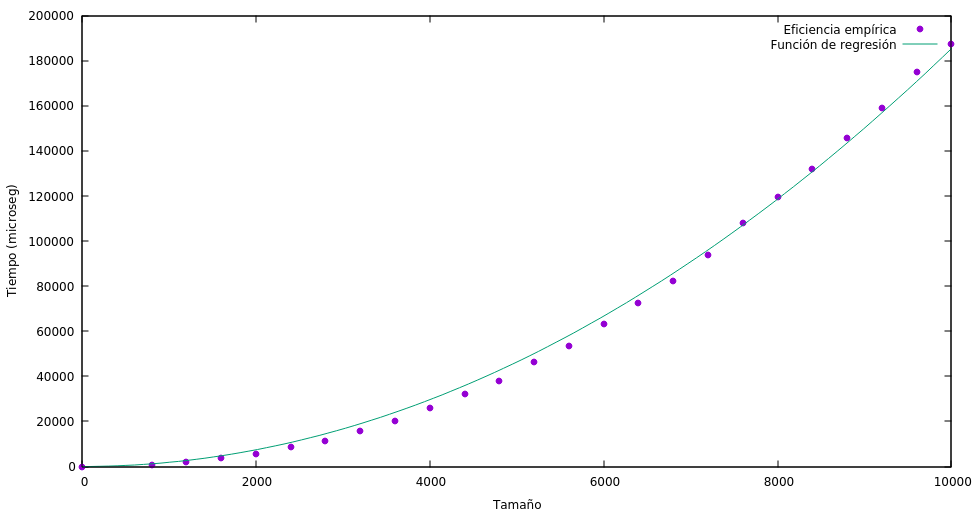
\includegraphics[scale=0.50]{burbuja_hibrida.png}
\caption{Cálculo de la eficiencia híbrida de burbuja}
\label{Eficiencia híbrida del algoritmo de burbuja}
\end{figure}

Sabiendo que la eficiencia teórica del algoritmo de burbuja es $\frac a2n^2+\frac{3a}{2}n+a\in O(n^2)$, se 
usó una curva de regresión cuadrática para aproximar los valores de la eficiencia teórica a la eficiencia
empírica. Podemos observar que se trata de una parábola cuya amplitud es inmensa. El ajuste tiene un
coeficiente de regresión con valor igual a 0.999776, por lo que podemos concluir que la eficiencia teórica
se ajusta a la perfección a los resultados obtenidos en la ejecución del algoritmo, pudiendo concluir deinitivamente que la eficiencia del algoritmo de burbuja es cuadrático.
\clearpage

%%%%%%%%%%%%%%%%%%%%%%%%%%%%%%%%%%%%%%%%%
%				GRÁFICAS				%
%%%%%%%%%%%%%%%%%%%%%%%%%%%%%%%%%%%%%%%%%
\section{Anexo: Gráficas de las eficiencias empíricas}

\begin{figure}[htp]
\centering
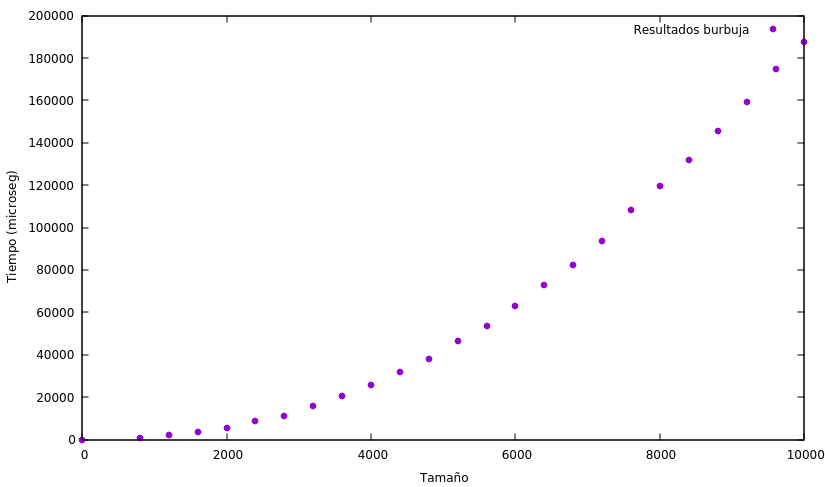
\includegraphics[scale=0.60]{burbuja_empirica.png}
\caption{Eficiencia empírica del algoritmo de burbuja}
\label{Gráfico de la eficiencia empírica del algoritmo de burbuja}
\end{figure}

\begin{figure}[htp]
\centering
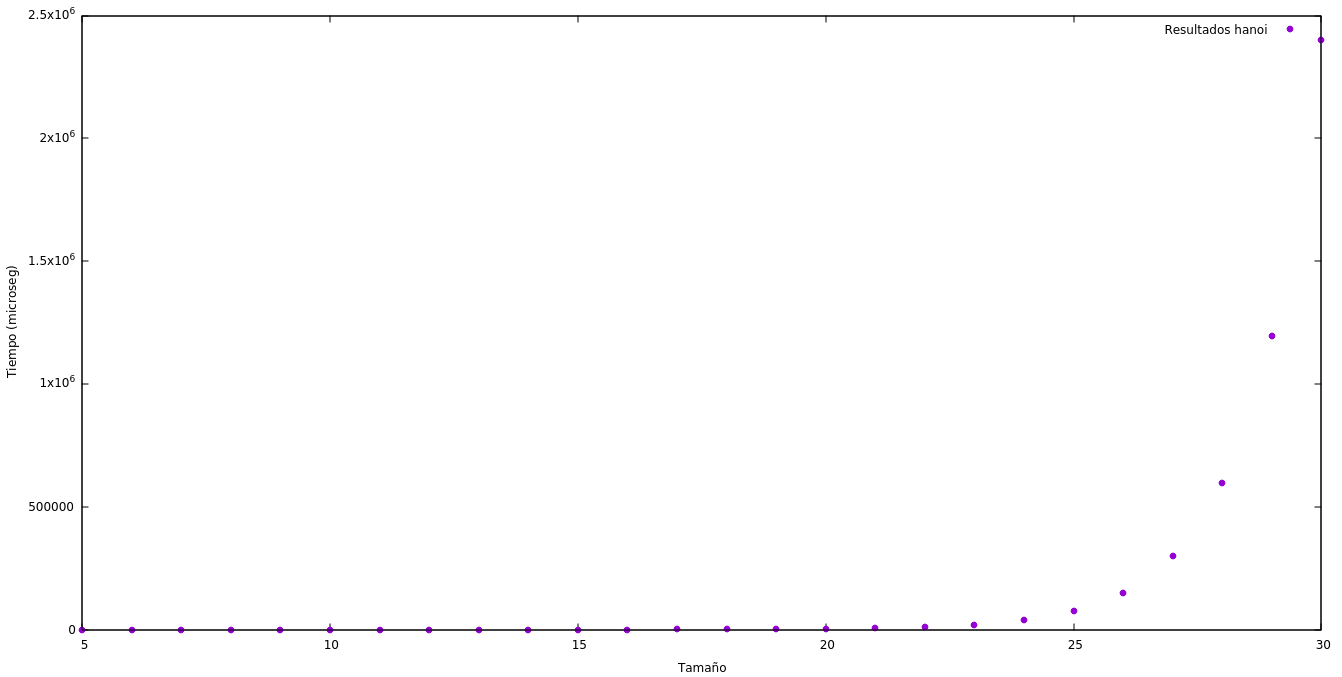
\includegraphics[scale=0.40]{hanoi_empirica.png}
\caption{Eficiencia empírica del algoritmo de hanoi}
\label{Gráfico de la eficiencia empírica del algoritmo de hanoi}
\end{figure}

\end{document}